\documentclass[a4paper,12pt]{article}

\usepackage[slovak]{babel}
\usepackage[left=1.5cm,text={18cm, 25cm},top=2cm]{geometry}
\usepackage[utf8]{inputenc}
\usepackage{times}
\usepackage{amsthm}
\usepackage{amsmath,amsfonts,amssymb}
\usepackage{graphicx}
\usepackage{rotating}
\usepackage{listings}
\usepackage{xcolor}
\usepackage{microtype}
\usepackage{textcomp}
\usepackage{caption}

\definecolor{codegreen}{rgb}{0,0.6,0}
\definecolor{codegray}{rgb}{0.5,0.5,0.5}
\definecolor{codepurple}{rgb}{0.58,0,0.82}
\definecolor{backcolour}{rgb}{0.95,0.95,0.92}

\lstdefinestyle{mystyle}{
    backgroundcolor=\color{backcolour},   
    commentstyle=\color{codegreen},
    keywordstyle=\color{magenta},
    numberstyle=\tiny\color{codegray},
    stringstyle=\color{codepurple},
    basicstyle=\ttfamily\footnotesize,
    breakatwhitespace=false,         
    breaklines=true,                 
    captionpos=b,                    
    keepspaces=true,                 
    numbers=left,                    
    numbersep=5pt,                  
    showspaces=false,                
    showstringspaces=false,
    showtabs=false,                  
    tabsize=2,
    extendedchars=false,
    escapeinside={\%*}{*)},
    inputencoding=utf8
}
\lstset{style=mystyle}

\author{Jakub Mĺkvy (xmlkvy00)\\Adam Múdry (xmudry01)}
\date{\today}
\title{\Large\bf Projekt -- IMS 2020/2021}

\begin{document}
\begin{titlepage}
	\begin{center}
	    \vspace*{+3cm}
		\Huge
		\textsc{Fakulta informačních technologií\\
		\huge Vysoké učení technické v~Brně}\\
		\vspace{\stretch{0.382}}    
	    {\LARGE{Dokumentácia\\Projekt č. 11 do predmetu \textit{Modelování a simulace}\\
		 \vspace{4mm}
		 \Huge\textbf{{Modely přírodních a ekologických katastrof\\(Lesné požiare)}}\\
		 \vspace{4mm}
		 2020/2021
		 }}
		 
		\vspace{\stretch{0.618}}
	\end{center}
	{\Large \hfill Jakub Mĺkvy (xmlkvy00)\\
	\today \hfill Adam Múdry (xmudry01)}
	
	\thispagestyle{empty}
    \setcounter{page}{0}
\end{titlepage}

\newpage

\tableofcontents

\newpage
\section{Úvod}
Úlohou tohto projektu bolo naprogramovať program (\textit{ims}), ktorý simuluje prírodné a ekologické katastrofy, v našom príade lesné požiare.
\\
\\
Zoznam odovzdaných súborov: 
\begin{lstlisting}
src/main.cpp src/map.hpp src/cell.hpp src/etc.hpp
Makefile
dokumentacia.pdf
README.md
\end{lstlisting}

\subsection{Preklad}
Program sa prekladá pomocou nástroja {\bf make} spusteného v koreni priečinku:
\begin{lstlisting}
make
\end{lstlisting}
alebo
\begin{lstlisting}
make build
\end{lstlisting}
\leavevmode\\
Pre vytvorenie ladiacej verzie programu použite príkaz:
\begin{lstlisting}
make build-debug
\end{lstlisting}
\leavevmode\\
Makefile spúšťa program \textbf{g++} s nasledujúcimi parametrami:
\begin{lstlisting}
--std=c++17 -Wall -Wpedantic [-O3|-g]
\end{lstlisting}
a linkuje vytvorené objektové súbory na knižnice pomocou:
\begin{lstlisting}
 -lglut -lGLU -lGL
\end{lstlisting}
\leavevmode\\
Vytvára sa spustiteľný súbor {\bf ims} na koreni priečinku.

\subsection{Použitie}
Príkaz na spustenie (GUI verzia):
\begin{lstlisting}
make run
\end{lstlisting}
alebo verzia pre terminál:
\begin{lstlisting}
make run-terminal
\end{lstlisting}
alebo priamo cez vygenerovaný spustiteľný súbor:
\begin{lstlisting}
./ims [-h|--help] [-g|--gui]
\end{lstlisting}
\begin{lstlisting}
%*Príznaky a argumenty*):
    -h, --help        %*Ukáže pomocnú hlášku*)
    -g, --gui         %*Zapne podrobný výpis*)
\end{lstlisting}
Pred použitím programu musí existovať jeho spustiteľný súbor.

\newpage
\section{Teória}
Lesný požiar sa v realite šíri a udržuje podľa veľkého množstva faktorov.
Zohľadnenie týchto faktorov vedie k extenzívnym ale presným modelom pre simuláciu.
Jedným z týchto modelov je \textbf{ABBAMPAU model}, ktorý zahŕňa faktory
\textit{výška, typ vegetácie, teplota, vlhkosť, typ horenia, dĺžka horenia,
smer vetra, sila vetra, horlavosť}.
Riadi sa štvorcovými bunkami a Moorovym algoritmom najbližších susedov
(algoritmus sa pozerá na štyroch hraničných a štyroch diagonálnych susedov).
Ďalší s extenzívnych modelov je Rothermelov model, ktorý sa sústreďuje na fyzické vlastnosti ohňa
a jeho propagáciu v poveternostných podmienkach.

\subsection{SSL}
\textbf{Secure Sockets Layer} (doslova vrstva bezpečných socketov) je protokol, resp. vrstva vložená medzi vrstvu transportnú (napr. \textbf{TCP/IP}) a aplikačnú (napr. \textbf{HTTP}), ktorá poskytuje zabezpečení komunikácie šifrovaním a autentifikáciu komunikujúcich strán. \cite{wiki_ssl}

\leavevmode\\\\
Ukážka HTTP \textit{GET} požiadavky pre získanie správ z určitého kanálu:
\begin{lstlisting}
GET /api/channels/<ID %*kanálu*)>/messages HTTP/1.1\r\n
Host: discord.com\r\n
Authorization: Bot <Token>\r\n
\r\n
\end{lstlisting}
\leavevmode\\
Ukážka HTTP \textit{POST} požiadavky pre odoslanie odpovedi na server:
\begin{lstlisting}
POST /api/channels/<ID %*kanálu*)>/messages HTTP/1.1\r\n
Host: discord.com\r\n
Authorization: Bot <Token>\r\n
Content-Type: application/json\r\n
Content-Length: <%*Dĺžka správy*)>\r\n
\r\n
{"content": "echo: %*<Meno používateľa> - <Správa>*)"}\r\n
\r\n
\end{lstlisting}


\newpage
\section{Implementácia}
Zadanie projektu som implementoval v jazyku C++ písaného v štandarde C++17. 

\subsection{Načítavanie argumentov}
Po spustení programu sa načítavajú argumenty zo štandardného vstupu (\textit{stdin}) pomocou funkcie
\begin{lstlisting}[language=C++]
void parseArgs(int& argc, char* argv[], bool& show_help, bool& verbose, std::string& token);
\end{lstlisting}
ktorá využíva knižnicu \textit{getopt.h} a jednotlivé načítané argumenty vráti do premenných z parametrov funkcie.

\subsection{Zahájenie SSL spojenia}
Po načítaní \textit{tokenu} a ostatných argumentov zo štandardného vstupu program naviaže SSL spojenie pomocou funkcie 
\begin{lstlisting}[language=C++]
int initConnection(SSL** ssl_return);
\end{lstlisting}
ktorá vracia ukazovateľ na štruktúru \textbf{SSL} využíva OpenSSL knižnice \textit{openssl/ssl.h}, \textit{openssl/err.h} a pár iných knižníc určených pre programovanie so sieťami ako napr. \textit{netinet/in.h}.
\cite{stackoverflow}

\subsection{Získavanie informácii}
Získanú \textit{SSL} štruktúru môžeme využiť v nasledujúcich funkciách
\begin{lstlisting}[language=C++]
int sendPacket(SSL* ssl, const char *buf);
std::string recieveResponse(SSL* ssl);
\end{lstlisting}
z ktorých prvá posiela naše \textit{GET} alebo \textit{POST} požiadavky na Discord API a druhá spracováva odpoveď a vráti ju vo forme \textit{std::string}. \cite{stackoverflow}
\\\\
Telo HTTP odpovede je vo formáte \textbf{JSON}, ktorý program spracuje pomocou funkcií zo štandardnej knižnice C++ \textbf{regex} a naplní štruktúry 
\begin{lstlisting}[language=C++]
struct Message; // id, user_id, channel_id, timestamp, username, content, ...
struct Channel; // id, guild_id, name, messages, ...
struct Guild;   // id, name, channels, ...
\end{lstlisting}
ktoré obsahujú dáta ako id, názvy a podobne a sú vzájomne napojené.

\subsection{Odpovedanie na správy používateľov}
Po načítaní všetkých potrebných informácii môže program začať načítavať správy z jednotlivých kanálov a odpovedať na ne. Toto sa deje v jednom \textbf{while} cykle. Program porovnáva lokálny čas a čas odoslania správy, získaný z \textit{JSON} odpovede Discord serveru. Ak je správa staršia ako porovnaný čas, program ju ignoruje - ak je však správa nová, program ju zaregistruje a pošle odpoveď na server. Program taktiež ignoruje správy, ktoré poslali iný boti.
\\\\
\textit{Isabot} odpovedá s krátkym oneskorením, aby nepresiahol limit HTTP požiadaviek určený z Discord API.

\newpage
\section{Testovanie}
Program som testoval manuálne pomocou 2 vlastných skupín a kanálov a vlastného Discord účtu. 
\\\\
\begin{figure}[htp]
    \centering
    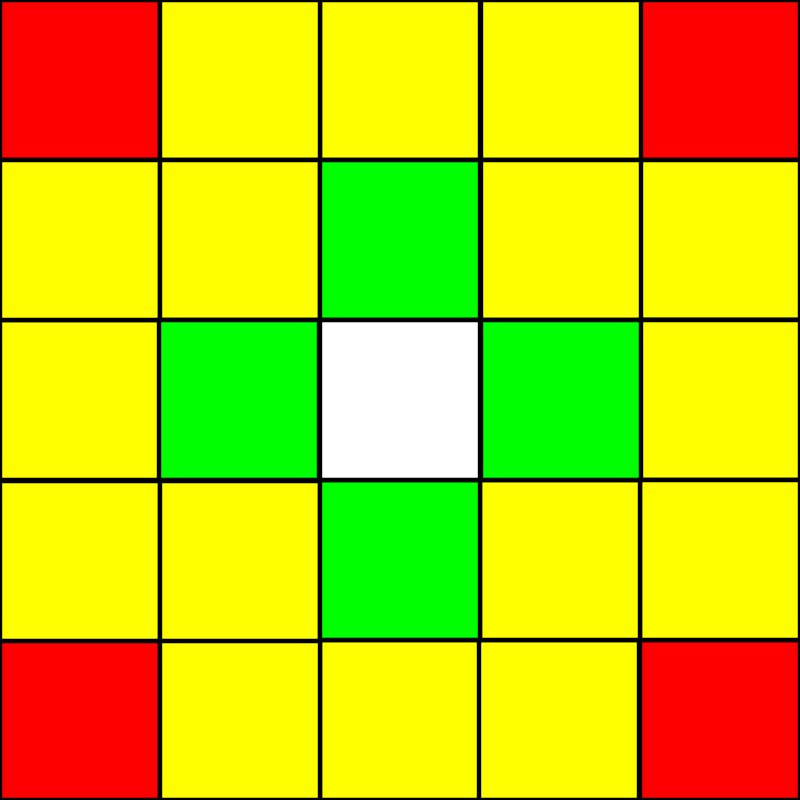
\includegraphics[width=10cm]{neighbor_radius.png}
    \captionsetup{justification=centering,margin=2cm}
    \caption{Zobrazenie vnímania vzdialenosti od bunky.\\\textit{Biela} - aktuálna bunka, \textit{zelená} - bunky (4) o vzdialenosti 1,\\\textit{žltá} - bunky (16) o vzdialenosti 2, \textit{červená} - bunky (4) o vzdialenosti 3.}
    \label{fig:neighbor_radius}
\end{figure}

\begin{figure}[htp]
    \centering
    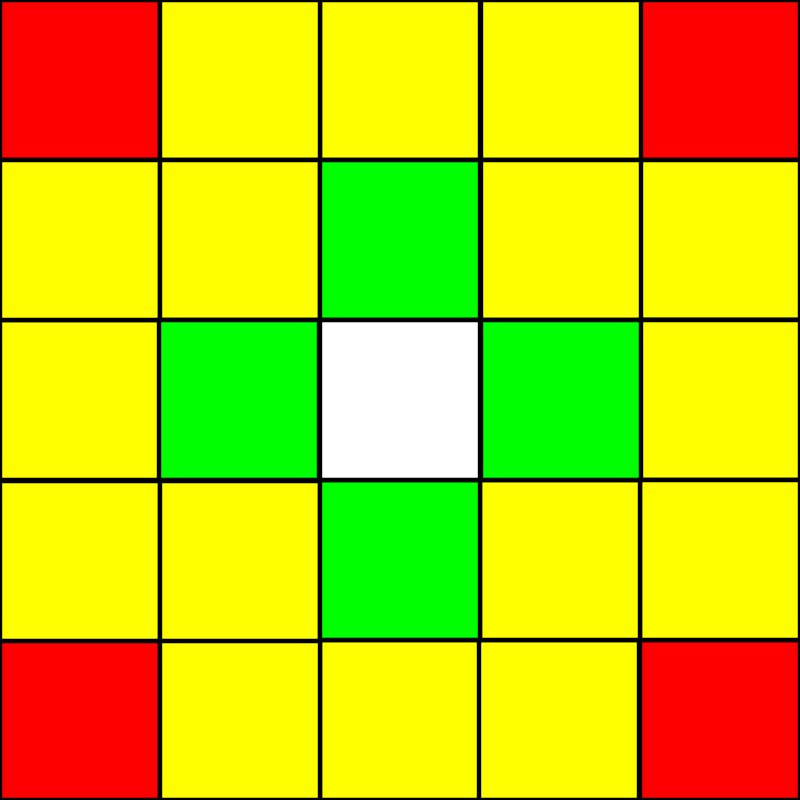
\includegraphics[width=10cm]{neighbor_radius.png}
    \captionsetup{justification=centering,margin=2cm}
    \caption{Zobrazenie vnímania vzdialenosti od bunky.\\\textit{Biela} - aktuálna bunka, \textit{zelená} - bunky (4) o vzdialenosti 1,\\\textit{žltá} - bunky (16) o vzdialenosti 2, \textit{červená} - bunky (4) o vzdialenosti 3.}
    \label{fig:neighbor_radius}
\end{figure}

\newpage
\section{Bibliografia}
\bibliographystyle{czechiso}
\bibliography{manual}
\nocite{CAmodel4FF}
\nocite{Pnoise}

\end{document}
